% Options for packages loaded elsewhere
\PassOptionsToPackage{unicode}{hyperref}
\PassOptionsToPackage{hyphens}{url}
%
\documentclass[
  english,
  man,floatsintext]{apa6}
\usepackage{lmodern}
\usepackage{amssymb,amsmath}
\usepackage{ifxetex,ifluatex}
\ifnum 0\ifxetex 1\fi\ifluatex 1\fi=0 % if pdftex
  \usepackage[T1]{fontenc}
  \usepackage[utf8]{inputenc}
  \usepackage{textcomp} % provide euro and other symbols
\else % if luatex or xetex
  \usepackage{unicode-math}
  \defaultfontfeatures{Scale=MatchLowercase}
  \defaultfontfeatures[\rmfamily]{Ligatures=TeX,Scale=1}
\fi
% Use upquote if available, for straight quotes in verbatim environments
\IfFileExists{upquote.sty}{\usepackage{upquote}}{}
\IfFileExists{microtype.sty}{% use microtype if available
  \usepackage[]{microtype}
  \UseMicrotypeSet[protrusion]{basicmath} % disable protrusion for tt fonts
}{}
\makeatletter
\@ifundefined{KOMAClassName}{% if non-KOMA class
  \IfFileExists{parskip.sty}{%
    \usepackage{parskip}
  }{% else
    \setlength{\parindent}{0pt}
    \setlength{\parskip}{6pt plus 2pt minus 1pt}}
}{% if KOMA class
  \KOMAoptions{parskip=half}}
\makeatother
\usepackage{xcolor}
\IfFileExists{xurl.sty}{\usepackage{xurl}}{} % add URL line breaks if available
\IfFileExists{bookmark.sty}{\usepackage{bookmark}}{\usepackage{hyperref}}
\hypersetup{
  pdftitle={QpFMRI: Bayesian adaptive stimulus presentation for real-time fMRI},
  pdfauthor={Steven M. Weisberg1 \& Geoffrey K. Aguirre2},
  pdflang={en-EN},
  pdfkeywords={adaptive stimulation, fMRI, Quest+, real-time fMRI, vision neuroscience},
  hidelinks,
  pdfcreator={LaTeX via pandoc}}
\urlstyle{same} % disable monospaced font for URLs
\usepackage{graphicx,grffile}
\makeatletter
\def\maxwidth{\ifdim\Gin@nat@width>\linewidth\linewidth\else\Gin@nat@width\fi}
\def\maxheight{\ifdim\Gin@nat@height>\textheight\textheight\else\Gin@nat@height\fi}
\makeatother
% Scale images if necessary, so that they will not overflow the page
% margins by default, and it is still possible to overwrite the defaults
% using explicit options in \includegraphics[width, height, ...]{}
\setkeys{Gin}{width=\maxwidth,height=\maxheight,keepaspectratio}
% Set default figure placement to htbp
\makeatletter
\def\fps@figure{htbp}
\makeatother
\setlength{\emergencystretch}{3em} % prevent overfull lines
\providecommand{\tightlist}{%
  \setlength{\itemsep}{0pt}\setlength{\parskip}{0pt}}
\setcounter{secnumdepth}{-\maxdimen} % remove section numbering
% Make \paragraph and \subparagraph free-standing
\ifx\paragraph\undefined\else
  \let\oldparagraph\paragraph
  \renewcommand{\paragraph}[1]{\oldparagraph{#1}\mbox{}}
\fi
\ifx\subparagraph\undefined\else
  \let\oldsubparagraph\subparagraph
  \renewcommand{\subparagraph}[1]{\oldsubparagraph{#1}\mbox{}}
\fi
% Manuscript styling
\usepackage{upgreek}
\captionsetup{font=singlespacing,justification=justified}

% Table formatting
\usepackage{longtable}
\usepackage{lscape}
% \usepackage[counterclockwise]{rotating}   % Landscape page setup for large tables
\usepackage{multirow}		% Table styling
\usepackage{tabularx}		% Control Column width
\usepackage[flushleft]{threeparttable}	% Allows for three part tables with a specified notes section
\usepackage{threeparttablex}            % Lets threeparttable work with longtable

% Create new environments so endfloat can handle them
% \newenvironment{ltable}
%   {\begin{landscape}\begin{center}\begin{threeparttable}}
%   {\end{threeparttable}\end{center}\end{landscape}}
\newenvironment{lltable}{\begin{landscape}\begin{center}\begin{ThreePartTable}}{\end{ThreePartTable}\end{center}\end{landscape}}

% Enables adjusting longtable caption width to table width
% Solution found at http://golatex.de/longtable-mit-caption-so-breit-wie-die-tabelle-t15767.html
\makeatletter
\newcommand\LastLTentrywidth{1em}
\newlength\longtablewidth
\setlength{\longtablewidth}{1in}
\newcommand{\getlongtablewidth}{\begingroup \ifcsname LT@\roman{LT@tables}\endcsname \global\longtablewidth=0pt \renewcommand{\LT@entry}[2]{\global\advance\longtablewidth by ##2\relax\gdef\LastLTentrywidth{##2}}\@nameuse{LT@\roman{LT@tables}} \fi \endgroup}

% \setlength{\parindent}{0.5in}
% \setlength{\parskip}{0pt plus 0pt minus 0pt}

% \usepackage{etoolbox}
\makeatletter
\patchcmd{\HyOrg@maketitle}
  {\section{\normalfont\normalsize\abstractname}}
  {\section*{\normalfont\normalsize\abstractname}}
  {}{\typeout{Failed to patch abstract.}}
\patchcmd{\HyOrg@maketitle}
  {\section{\protect\normalfont{\@title}}}
  {\section*{\protect\normalfont{\@title}}}
  {}{\typeout{Failed to patch title.}}
\makeatother
\shorttitle{Bayesian adaptive fMRI}
\keywords{adaptive stimulation, fMRI, Quest+, real-time fMRI, vision neuroscience\newline\indent Word count: X}
\usepackage{lineno}

\linenumbers
\usepackage{csquotes}
\usepackage{setspace}
\captionsetup[figure]{font={stretch=1,scriptsize}}
\usepackage{amsmath}
\ifxetex
  % Load polyglossia as late as possible: uses bidi with RTL langages (e.g. Hebrew, Arabic)
  \usepackage{polyglossia}
  \setmainlanguage[]{english}
\else
  \usepackage[shorthands=off,main=english]{babel}
\fi

\title{QpFMRI: Bayesian adaptive stimulus presentation for real-time fMRI}
\author{Steven M. Weisberg\textsuperscript{1} \& Geoffrey K. Aguirre\textsuperscript{2}}
\date{}


\authornote{

Steven M. Weisberg, University of Florida, Department of Psychology
Geoffrey K. Aguirre, University of Pennsylvania, Department of Neurology, Center for Cognitive Neuroscience.
Pre-print submitted for peer review.

Correspondence concerning this article should be addressed to Steven M. Weisberg, 945 Center Dr., Gainesville, FL 32611. E-mail: \href{mailto:stevenweisberg@ufl.edu}{\nolinkurl{stevenweisberg@ufl.edu}}

}

\affiliation{\vspace{0.5cm}\textsuperscript{1} University of Florida\\\textsuperscript{2} University of Pennsylvania}

\abstract{
QUEST+ (Q+, Watson, 2017) is an adaptive stimulus selection approach that works to minimize uncertainty in a parameterized model of the responses. Unlike random stimulus selection, Q+ stimulus selection dynamically select the next stimulus based upon the prior responses of the subject, and an underlying stimulus-response model. While this approach has been successful in behavioral experiments, to use Q+ in BOLD fMRI experiments, experimenters require a `real-time' measure of the BOLD response to stimuli as they are presented and solutions that address idiosyncracies of the BOLD signal. We have created a software toolbox that 1) extracts (or simulates) the BOLD fMRI signal from a brain region as imaging volumes are acquired, 2) cleans and fits the growing time-series to estimate the response on each trial, and 3) applies Q+ to the responsees to select the next stimulus. In simulations that model empirical data for a simple visual contrast experiment featuring stimuli of varying visual contrast values, we found that Q+ stimulus selection recovers model parameters more accurately than random stimulus selection. We report the results of stimulus selection approaches on simulated data, as well as how to optimize experimental parameters (e.g., TR, trial length) to improve model fit. In addition, we describe our solutions to the technical challenges posed by adapting Q+ for fMRI data, describe the codebase we have written to implement the solution, and present sample uses for Q+ stimulus selection in future real-time BOLD fMRI experiments.
}



\begin{document}
\maketitle

Introductory text placeholder.

\hypertarget{general-background-of-the-problem}{%
\subsection{General background of the problem}\label{general-background-of-the-problem}}

\hypertarget{specific-problem-to-be-solved}{%
\subsection{Specific problem to be solved}\label{specific-problem-to-be-solved}}

\hypertarget{here-we}{%
\subsection{Here we \ldots{}}\label{here-we}}

\hypertarget{method}{%
\section{Method}\label{method}}

\hypertarget{approach}{%
\subsection{Approach}\label{approach}}

Does the qpfMRI approach yield improved fit over random stimulus selection? As a proof of principle, we created a forward of model primary visual cortical function using a logistic model (Equation 1). We selected this model because it is relatively simple (only two parameters vary between 0 and 1) and because logistic functions would be a plausible model for visual cortex (e.g., in response to light flickering at varying frequencies) and thus would make a good neurometric function. That is, a logistic function can model the increasing neural signal in response to an increase in stimulus flicker. Let \emph{slope} equal the slope of the curve at the semi-saturation point. Let \emph{semiSat} equal the point on the x-axis at which the y-axis reaches 50\%.Let \(x_0\) be the value of a stimulus. Then, the logistic function is defined as:
\begin{equation}
  y_0 = 1-\frac{1}{(e^{(slope*(x_0-semiSat)})}
  \end{equation}
We developed a closed-loop pipeline, starting from known model parameters and resulting in an estimate of those same parameters from simulated BOLD fMRI data. The broad steps were as follows. 1) Select a set of model parameters for the logistic function. 2) Simulate BOLD fMRI data in response to stimuli based on the known model parameters. 3) Use a forward model to generate simulated BOLD fMRI data. 4) Use a reverse model to obtain estimates of the BOLD response for each trial. 4) Select the next stimulus based on either random stimulus selection (control) or applying Q+ to the responses.
In developing simulations to achieve this goal, we solved several problems in applying Q+ to BOLD fMRI data. To wit: BOLD fMRI data are (1) continuous, (2) noisy, (3) unitless, (4) have a maximum response that is unknown \emph{a priori} and (5) are subject to low-frequency temporal variation. We address each of these in turn, but first provide a general overview of Q+.

\hypertarget{quest}{%
\subsection{Quest +}\label{quest}}

Q+ (David H. Brainard, 2017; Watson, 2017) is a multidimensional Bayesian method for adaptive stimulus presentation. Q+ operates by computing the conditional probability of a behavioral outcome for each set of stimulus parameters. Q+ is a generalization on QUEST (Watson \& Pelli, 1983), which estimates a psychometric function on the basis of a single stimulus dimension and provides an adaptive testing procedure to fit the function. Whereas QUEST could only compute one stimulus dimension, one psychometric function parameter, and two outcome measures, Q+ allows for multiple stimulus dimensions, psychometric parameters, and many outcome measures. Here, we further expand Q+ to model the BOLD fMRI signal based on a neurometric function, which fits stimulus dimensions to changes in the BOLD response. To help explain, we contrast a BOLD fMRI experiment with a color categorization behavioral experiment. In the color category experiment, a participant is presented with one patch of color of varying wavelengths at a time and must select which color category (e.g., red, blue, green, or yellow), the color belongs to.

\hypertarget{challenge-1-the-bold-signal-is-continuous}{%
\subsubsection{Challenge 1: The BOLD signal is continuous}\label{challenge-1-the-bold-signal-is-continuous}}

Q+ operates over discrete categorical outcomes, such as selecting amongst a set of color names for a stimulus. For stimuli in the middle of the red spectrum, roughly 100\% of responses will be \enquote{red.} But as the color patch drifts closer to yellow, this percentage will decrease. But the \enquote{outcomes} for the BOLD fMRI signal are continuous. There is no principled way to divide the BOLD signal up into categories, and arbitrarily small categories will increase computation time dramatically. To solve this, we define a fixed number of outcome categories onto which we map the amplitude of the BOLD response.

\hypertarget{challenge-2-the-bold-signal-is-noisy-and-outcomes-are-sparse}{%
\subsubsection{Challenge 2: The BOLD signal is noisy and outcomes are sparse}\label{challenge-2-the-bold-signal-is-noisy-and-outcomes-are-sparse}}

Q+ esimtates parameters of a function that predict the proportion of trial outcomes that fall in each category. For example, from wavelength (the stimulus dimension) Q+ will generate a prediction for the percentage of trials that will be described as red, green, blue, or yellow. Although there is uncertainty in the response over trials (i.e., presented with the same wavelength patch, participants will sometimes call the color red and other times call the color green), each individual response is assumed to be certain. That is, we do not assume that a participant who has said \enquote{green} means to say \enquote{red} 10\% of the time. The BOLD signal, on the other hand, is noisy. In response to a given stimulus, the BOLD signal will assume a range of values, normally distributed around the population mean (given some assumptions.) That is, the BOLD signal is a response that itself has uncertainty built in. In other words, physiologic noise in the BOLD fMRI response causes outcomes to be spread across categories around the veridical response value. Given unlimited amounts of data, this would not be a problem because the mean value of the BOLD response for a given stimulus would converge on the true value. But, unlike the color study, which could have 100s of trials, BOLD fMRI trials typically number in the 10s, thus responses are potentially sparse across the many outcome categories. To solve this, the outcome for each stimulus is determined by the parameters oof the neurometric function, plus a parameter we call \(\sigma\) (\emph{sigma}) that controls the width of a Gaussian that distributes outcomes across adjacent categories. Q+ estimates the value of \(\sigma\) as well.

\hypertarget{challenge-3-the-bold-fmri-signal-is-unitless.}{%
\subsubsection{Challenge 3: The BOLD fMRI signal is unitless.}\label{challenge-3-the-bold-fmri-signal-is-unitless.}}

Q+ operates on outcomes with defined boundaries. The BOLD fMRI signal is unitless and thus interpreted relative to a baseline stimulus. To solve this, the outcome amplitude is calculated relative to a specified baseline stimulus, which is required to be presented at the beginning of the experiment.

\hypertarget{challenge-4-the-maximum-response-is-not-known-a-priori}{%
\subsubsection{\texorpdfstring{Challenge 4: The maximum response is not known \emph{a priori}}{Challenge 4: The maximum response is not known a priori}}\label{challenge-4-the-maximum-response-is-not-known-a-priori}}

Similarly, the maximum possible response is not known \emph{a priori} and must be calculated from the neurometric curve. Again, Q+ operates on outcomes with defined boundaries, so we must impose a possible range on the BOLD signal from baseline to maximum. To solve this, the outcome algorithm adjusts the mapping of BOLD fMRI response to the outcome categories, updating an estimate of maximum BOLD response.

\hypertarget{challenge-5-bold-fmri-data-are-subject-to-low-frequency-temporal-noise}{%
\subsubsection{Challenge 5: BOLD fMRI data are subject to low-frequency temporal noise}\label{challenge-5-bold-fmri-data-are-subject-to-low-frequency-temporal-noise}}

Q+ accumulates evidence across trials. To obtain the amplitude of response on a new trial, the growing BOLD fMRI signal is subject to pre-processing, including the removal of low-frequency noise. This calculation alters the estimated response to prior trials. To solve this, we iteratively re-train Q+ with all past trials up through the current trial.

\hypertarget{qpfmri-an-overview}{%
\subsection{QPFMRI: An overview}\label{qpfmri-an-overview}}

The QPfMRI pipeline is detailed in Figure 1. We describe the pipeline with simulated BOLD fMRI data where the model parameters can be specified in advance, but the principles for implementing Q+ with real BOLD fMRI data will be similar. To summarize, we specify a set of model parameters (Fig. 1A) then select trials and calculate the estimated BOLD fMRI response based on the model with added simulated physiologic noise. This results in a BOLD fMRI timeseries (Fig. 1B), from which we calculate the estimated response to each trial. We then pass the series of trials and outcomes to Q+ (Fig. 1C), which provides an adaptive suggestion for the next trial. Finally, at the end of the simulation, we estimate model fit (Fig. 1E).

\newpage
\begin{figure}

{\centering \includegraphics[width=300px]{figures/Figure1} 

}

\caption{An overview of the processing pipeline in converting a BOLD signal to a Quest+ outcome. A set of model parameters is chosen (A), resulting in a predicted value for the BOLD signal, normalized between 0 and 1. Trials are then selected from this curve, which can be baseline trials (light grey dot), where the expected BOLD response is expected to be the minimum. From these trials, a BOLD fMRI timeseries is simulated using the temporal fitting engine's forward model (B), which convolves the predicted neural response from the logistic function with a canonical hemodynamic function. Gaussian noise and pink noise are then added to this signal to simulate the physiologic noise typical of fMRI. The timeseries is then fit with a general linear model, resulting in the estimated response for each trial (green bands). The baseline response (light grey vertical panels) is estimated from the average of baseline trials, and the maximum BOLD response is also estimated (dark grey vertical panels) either from maximum BOLD trials or from the estimated maximum BOLD response based on the logistic curve. Then the Q+ outcome categories are created and each non-baseline and maximum BOLD trial is assigned to the outcome category that contains its estimated value. The bin numbers and outcome categories are then passed to Q+ (C), which calculates the conditional probabilities of the parameter values (the parameter space (D)), and returns a suggestion for the next trial to present, with the aim of minimizing the entropy among the choices in the parameter space. Finally, we estimate the best fitting model to the data, resulting in an estimate of each model parameter (E).
\newpage}\label{fig:methods-figure}
\end{figure}




\hypertarget{simulation-method}{%
\subsection{Simulation method}\label{simulation-method}}

\hypertarget{forward-model}{%
\subsubsection{Forward model}\label{forward-model}}

For the forward model, we selected sample parameters that we expected to be well behaved (e.g., yield values between 0 and 1 for most of their range). Our choice of logistic function parameters and the domain of possible parameter values to search through were fixed through all simulations except where otherwise noted.
We explain the flow of data using random stimulus selection. First, a random set of stimulus values is chosen of length \emph{N} (where N is the number of trials in the experiment). We also enforce a set number of baseline trials (where the expected BOLD response will be minimal) and maximum BOLD trials (where the expected BOLD signal will be maximal). Next, each stimulus value is passed to the logistic function using our chosen function parameters. The output of that function (which has been normalized to be between 0 for baseline and 1 for maximum response) is then convolved with a canonical hemodynamic response function and adding 1/f noise (pink noise, consistent with BOLD signal). We also add white noise to the simulated timeseries (the amount of white noise varied across simulations). The resulting continuous timeseries is then downsampled to match the number of TRs per trial in the simulation and mean-centered. These steps were implemented with the temporal fitting engine (\url{https://github.com/gkaguirrelab/temporalFittingEngine}).

\hypertarget{reverse-model}{%
\subsubsection{Reverse model}\label{reverse-model}}

In the real-time simulation, the continuous timeseries is fed into the reverse model one trial at a time. Each pass through the reverse model, the signal is mean-centered. The timeseries is also reference coded, meaning all baseline trials are averaged and that average is subtracted from the rest of the timeseries so that the minimum value (theoretically) is zero. Next, we apply a general linear model (GLM) in which the baseline trials are the baseline and every other trial is represented as a boxcar (a vector of length \emph{N*t} with zeros everywhere except the cells for that trial, which contain ones). The GLM is fit to the timeseries and the betas returned are then assigned to outcome categories. At the end of each trial, the logistic function parameter values are estimated and compared to the veridical logistic function parameters.
Timeseries cleaning (baseline and max BOLD), assigning outcomes, high-pass and low-pass filtering, removing linear drift, mean-centering.

\hypertarget{q-stimulus-selection}{%
\subsubsection{Q+ stimulus selection}\label{q-stimulus-selection}}

In behavioral experiments, the combinations of parameters are those that define the model. Due to the challenges listed above for fMRI, two additional parameters are searched for by Q+, which we call \emph{sigma} and \emph{beta}. Sigma can be thought of as the estimate of the noise in the BOLD fMRI signal, though it is implemented as the spread along the possible outcome categories (e.g., a small value of sigma means that one stimulus value will correspond to only a few possible outcome categories). Beta is a scaling parameter that is used to help estimate what the maximum BOLD response is and approaches 1 as the maximum BOLD response is better estimated.
For each stimulus - outcome category pair, Q+ updates the log-likelihood for all possible combinations of parameters. Depending on the previous stimuli, Q+ will select the next stimulus by determining which result will most reduce the remaining entropy in the set of parameter combinations.

\hypertarget{simulation-parameters}{%
\subsubsection{Simulation parameters}\label{simulation-parameters}}

In addition to the model parameters, which Q+ attempts to find, we also explore a range of simulation parameters. These include one parameter related to Q+ search, the number of outcome categories (7 or 15). Other parameters we explored relate to the structure of the simulation itself: simulated noise (the amount of white noise added to the simulated BOLD fMRI signal), the length of individual trials (8 or 12 seconds), the length of the TR (800 or 1600 ms).

We did not vary several other parameters, including the stimulus domain (which stimulus values could be selected), the value for the maximum BOLD response, and the proportion of outcome categories reserved for the top and bottom (which we call headroom and set at 10\%). We also did not vary the model parameter domains (i.e., the values that each model parameter could take on). We arrived at these choices through trial and error, which is a compelling reason itself to use the Q+ fMRI simulation toolbox to set parameters for fMRI experiments. Some choices (like increasing the number of outcome categories, or the size of the parameter and stimulus domains) drastically increase the time to run Q+, limiting its utility in real-time fMRI experiments. Others, like the choice of headroom, yield strange or nonsensical results if they are set too low (0\%) or too high (50\%).

\hypertarget{data-and-code-availability}{%
\subsubsection{Data and code availability}\label{data-and-code-availability}}

The data and code for the analyses described in the results is available in a git repository (\url{https://github.com/smweis/Weisberg_and_Aguirre_2020}). The QpfMRI toolbox is available for download and use (\url{https://github.com/smweis/qpfmri}).

\hypertarget{results}{%
\section{Results}\label{results}}

Our main approach is to compare simulated BOLD fMRI data timeseries that were generated using random stimulus selection with timeseries that were generated with Q+ optimization. We first step through one sample simulation, showing trial-by-trial results. We then describe simulations over a range of parameters comparing random stimulus selection with Q+ stimulus selection. The results demonstrate improved convergence on model parameters when Q+ controls stimulus selection. The results also suggest optimal parameters for real-time fMRI design using Q+ for TR and trial duration.

First, we describe one set of 100 6-minute simulated fMRI runs comparing Q+ with random stimulus selection for one set of model parameters and one set of simulation parameters. The first set of simulations illustrate the advantage of Q+ stimulus selection in the case of simulation parameters that optimize for realistic and desired fMRI conditions (fast TR, long trials, medium noise) and fast Q+ performance (few outcome categories).Next, we evaluate the range of performance for Q+ compared to random stimulus selection across a several control parameter choices. Finally, we explore performance within one set of control parameters across a range of model parameters.

For these next sets of simulations, we used the following control parameters: TR = 800ms; number of trials = 30; trial length = 12s. We set the estimated maximum BOLD to 1.5\% signal change and initialized the maximum BOLD value to 1\%. We enforced baseline and maximum BOLD trials to alternate for the first six trials and then mandated a baseline trial every subsequent 5th trial and a maximum BOLD trial every 10th trial. We chose the lowest level of noise (.05 SD).

\hypertarget{simulating-one-set-of-model-parameters}{%
\subsection{Simulating one set of model parameters}\label{simulating-one-set-of-model-parameters}}

To determine whether Q+ improves model fit over random stimulus selection, we selected model parameters and control parameters that we expected would behave well. We chose model parameters from the middle of the distribution (slope = .41, semi-saturation = .57), and which led to high differentiation among our stimulus domain. That is, variation in the range of possible stimulus values would lead to a unique model parameter solution, which would be discoverable by the Q+ algorithm. As stated above, we chose control parameters optimizing for desired fMRI conditions. The results of the simulations are summarized in Figure 2, Figure 3, and Figure 4. Qualitatively, Q+ stimulus selection led to a narrower distribution around the model parameters (Figure 2), with fewer outlying results. Q+ stimulus selection led to a higher overall fit as measured by R-squared (Figure 3). Over 50 simulations per type, the fit for Q+ stimulus selection was significantly higher, Wilcoxon signed-rank test Z(98) = 5.13, p \textless{} 0.0001 (Q+: \emph{M} = 0.9986, \emph{SD} = 0.0012; Random: \emph{M} = 0.9817, \emph{SD} = 0.0348).

\newpage

\begin{figure}
  
  {\centering 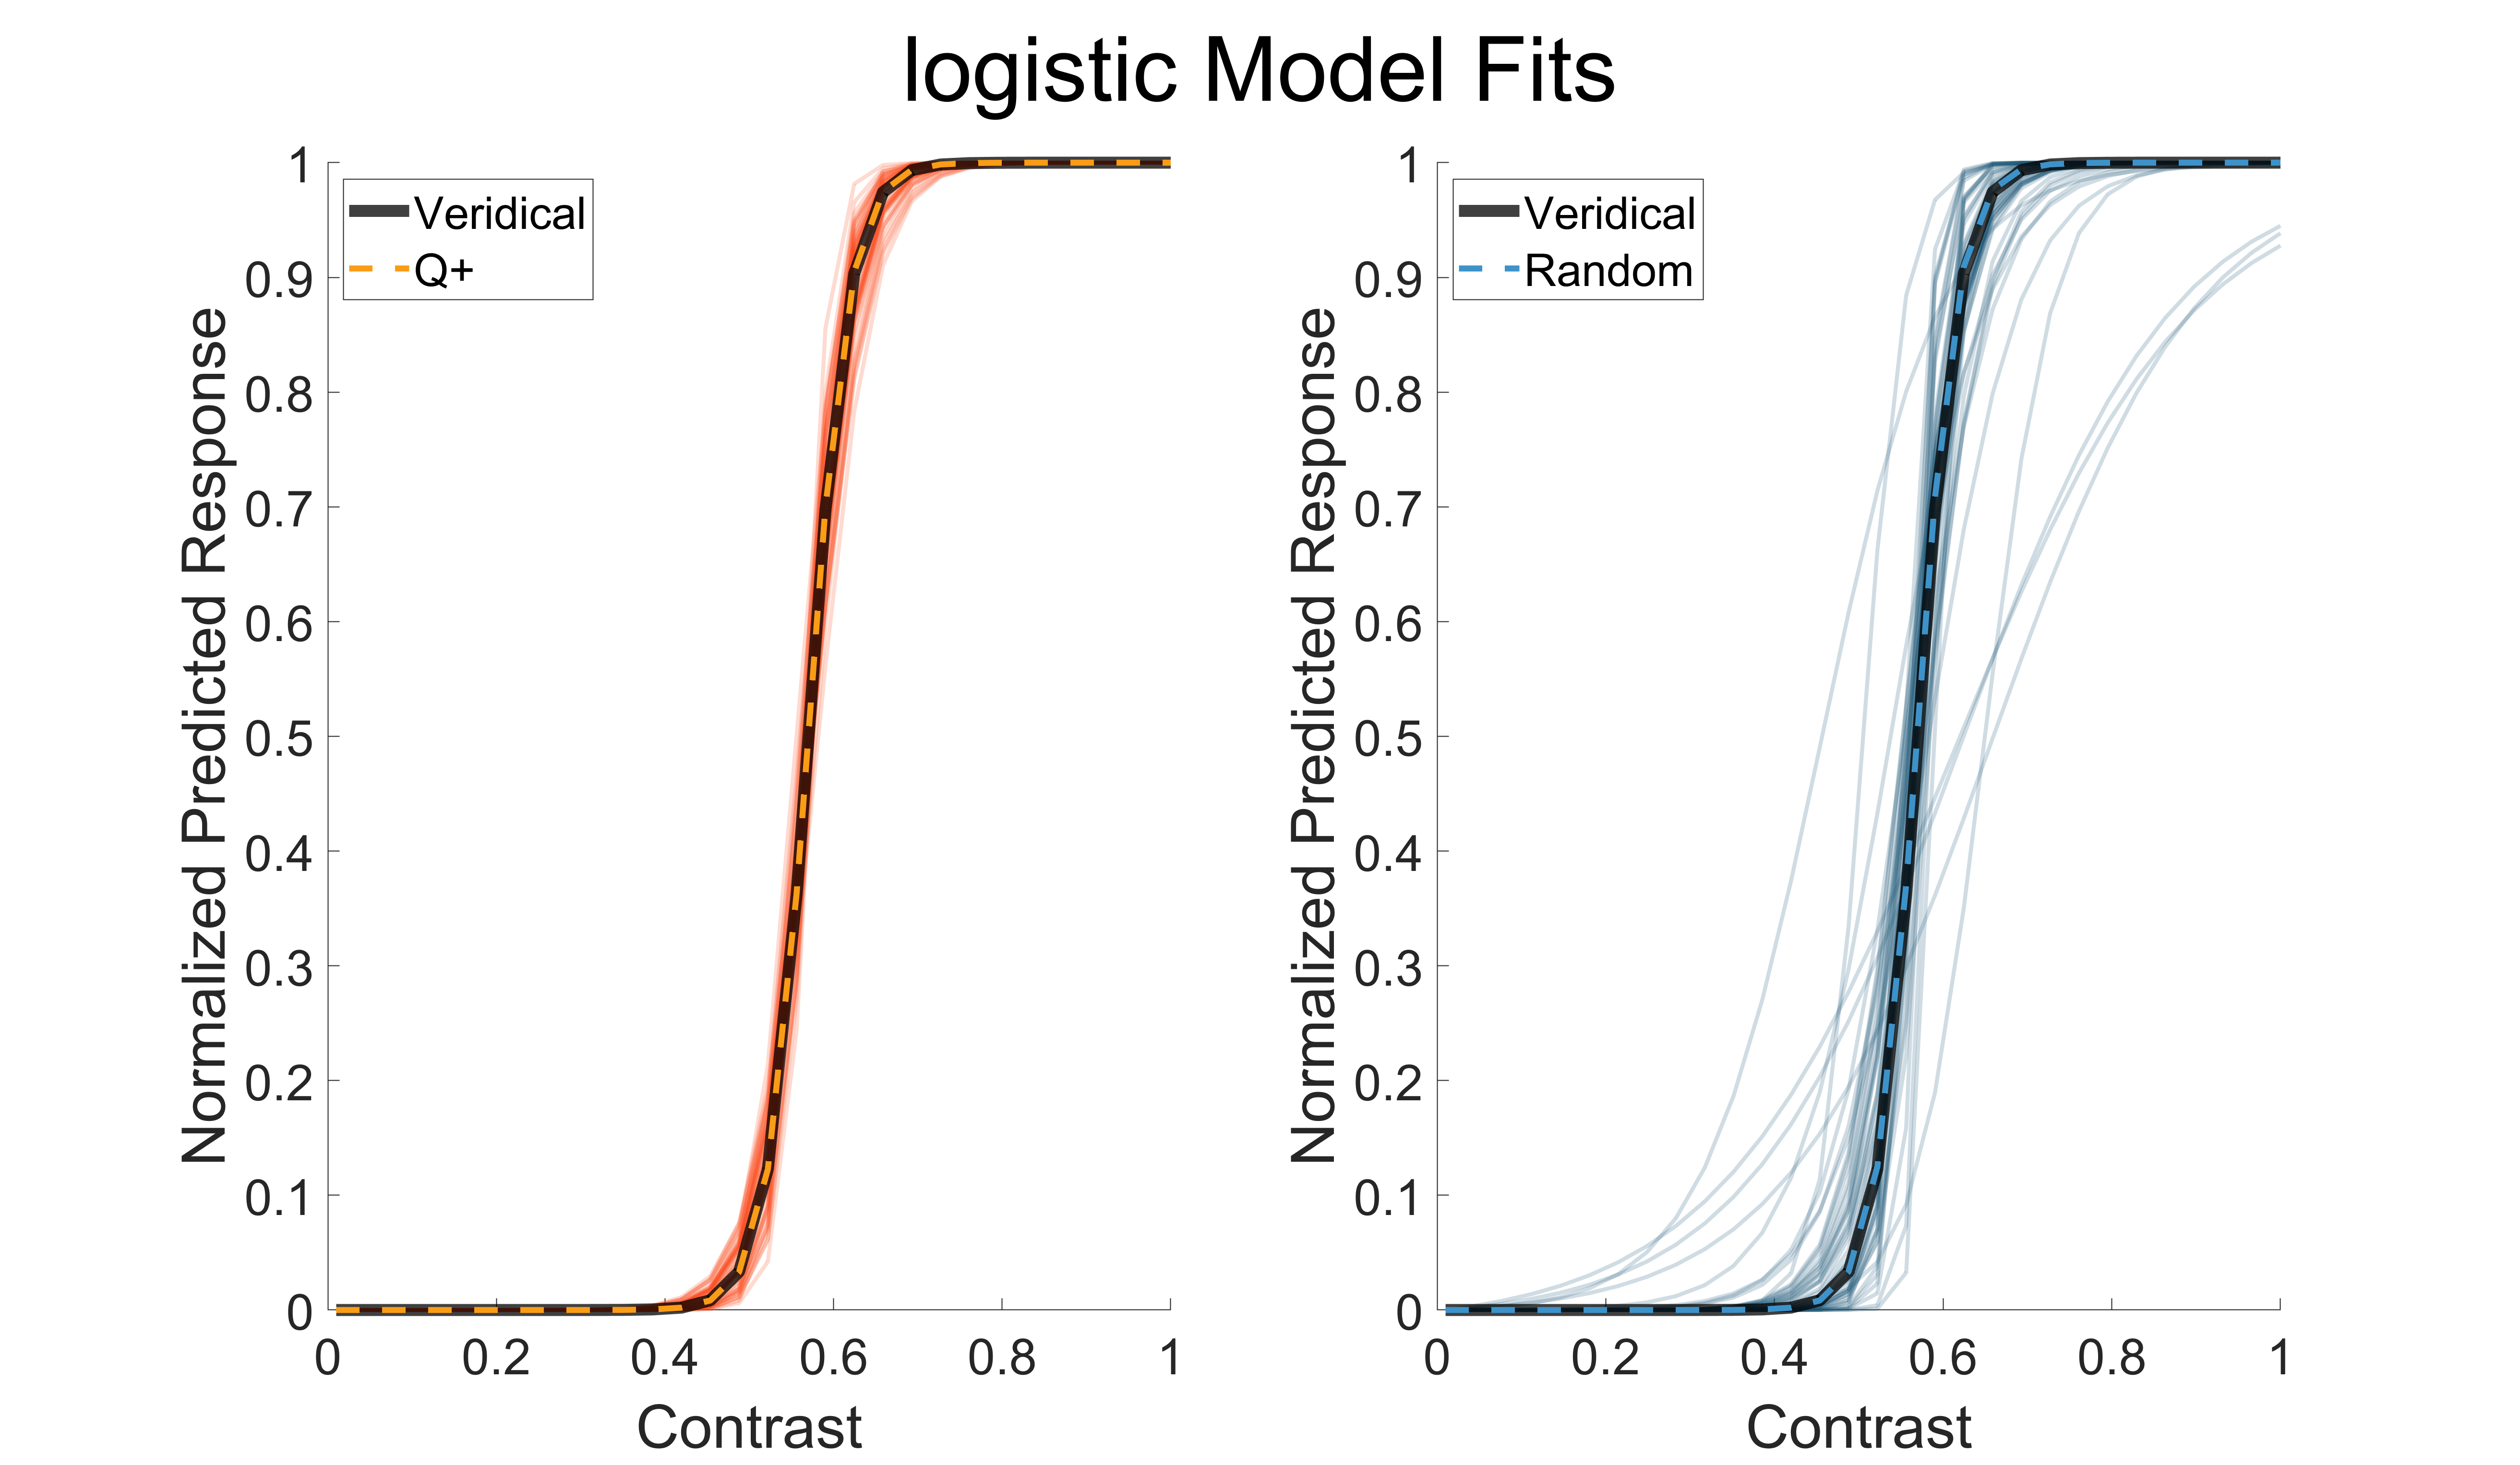
\includegraphics[width=500px]{../results/figs/fig1_7Outcomes_15Noise_12trialLength_800TR} 
  
  }
  
  \caption{The first set of simulations we evaluated are plotted. Each black line represents the veridical model (slope = .41, semi-saturation = .57) normalized to be between 0 and 1. Thin orange and blue lines represent each simulation's final parameters and the thick dotted line represents the mean of all 50 simulations. Although the average fit matched the veridical parameters for both Q+ (orange, right panel) and random (blue, left panel) stimulus selection, the resulting spread of parameter fits is visibly narrower for Q+.
\newpage}\label{fig:results-figure-firstsims-1}
  \end{figure}




\newpage

\begin{figure}
  
  {\centering 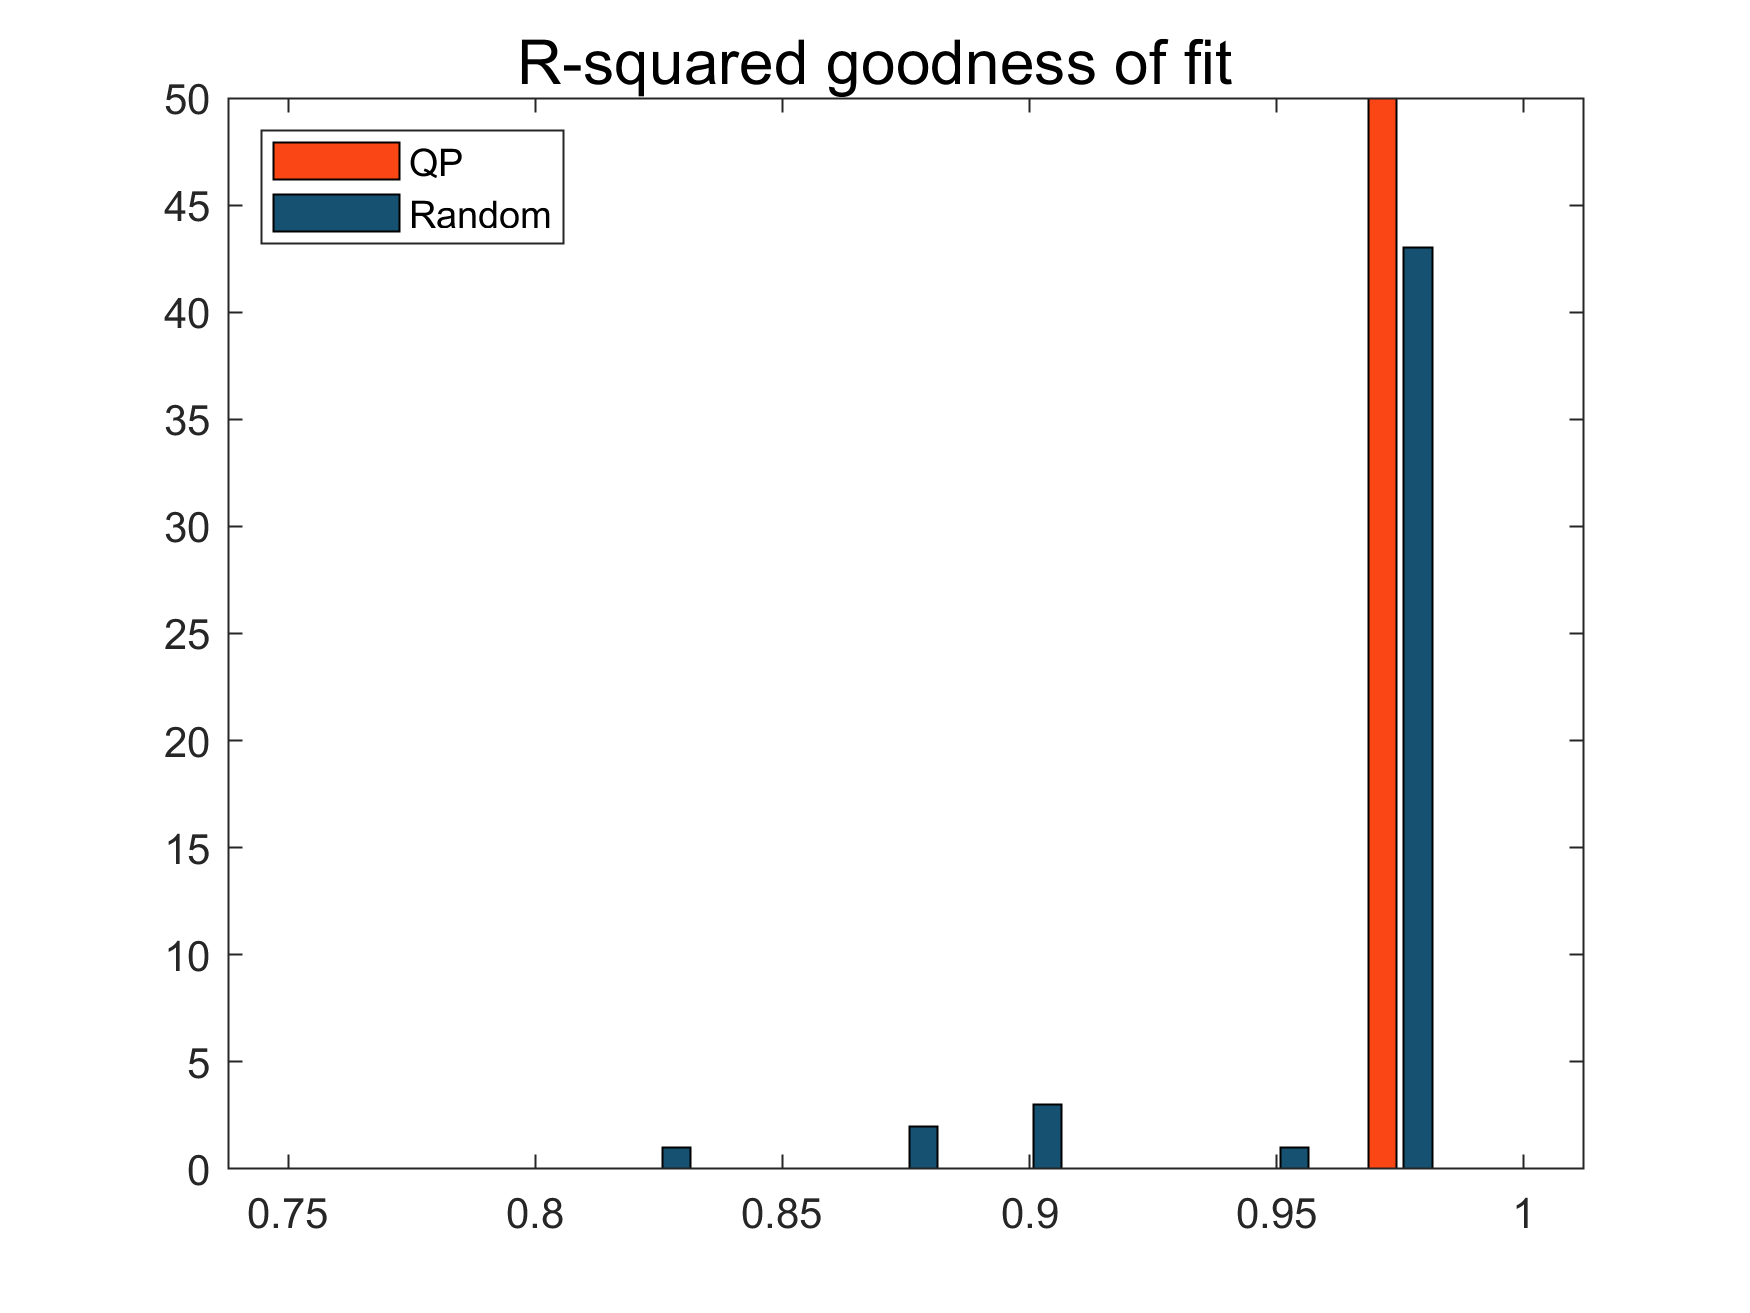
\includegraphics[width=500px]{../results/figs/fig2_7Outcomes_15Noise_12trialLength_800TR} 
  
  }
  
  \caption{To evaluate how well the resulting parameters matched the veridical parameters we calculated the squared Pearson's correlation between the output for each simulation with the output for the veridical parameters. This histogram depicts the results of each correlation for all Q+ (orange) and random (blue) stimulus selection simulations.
\newpage}\label{fig:results-figure-firstsims-2}
  \end{figure}




\newpage

\begin{figure}
  
  {\centering 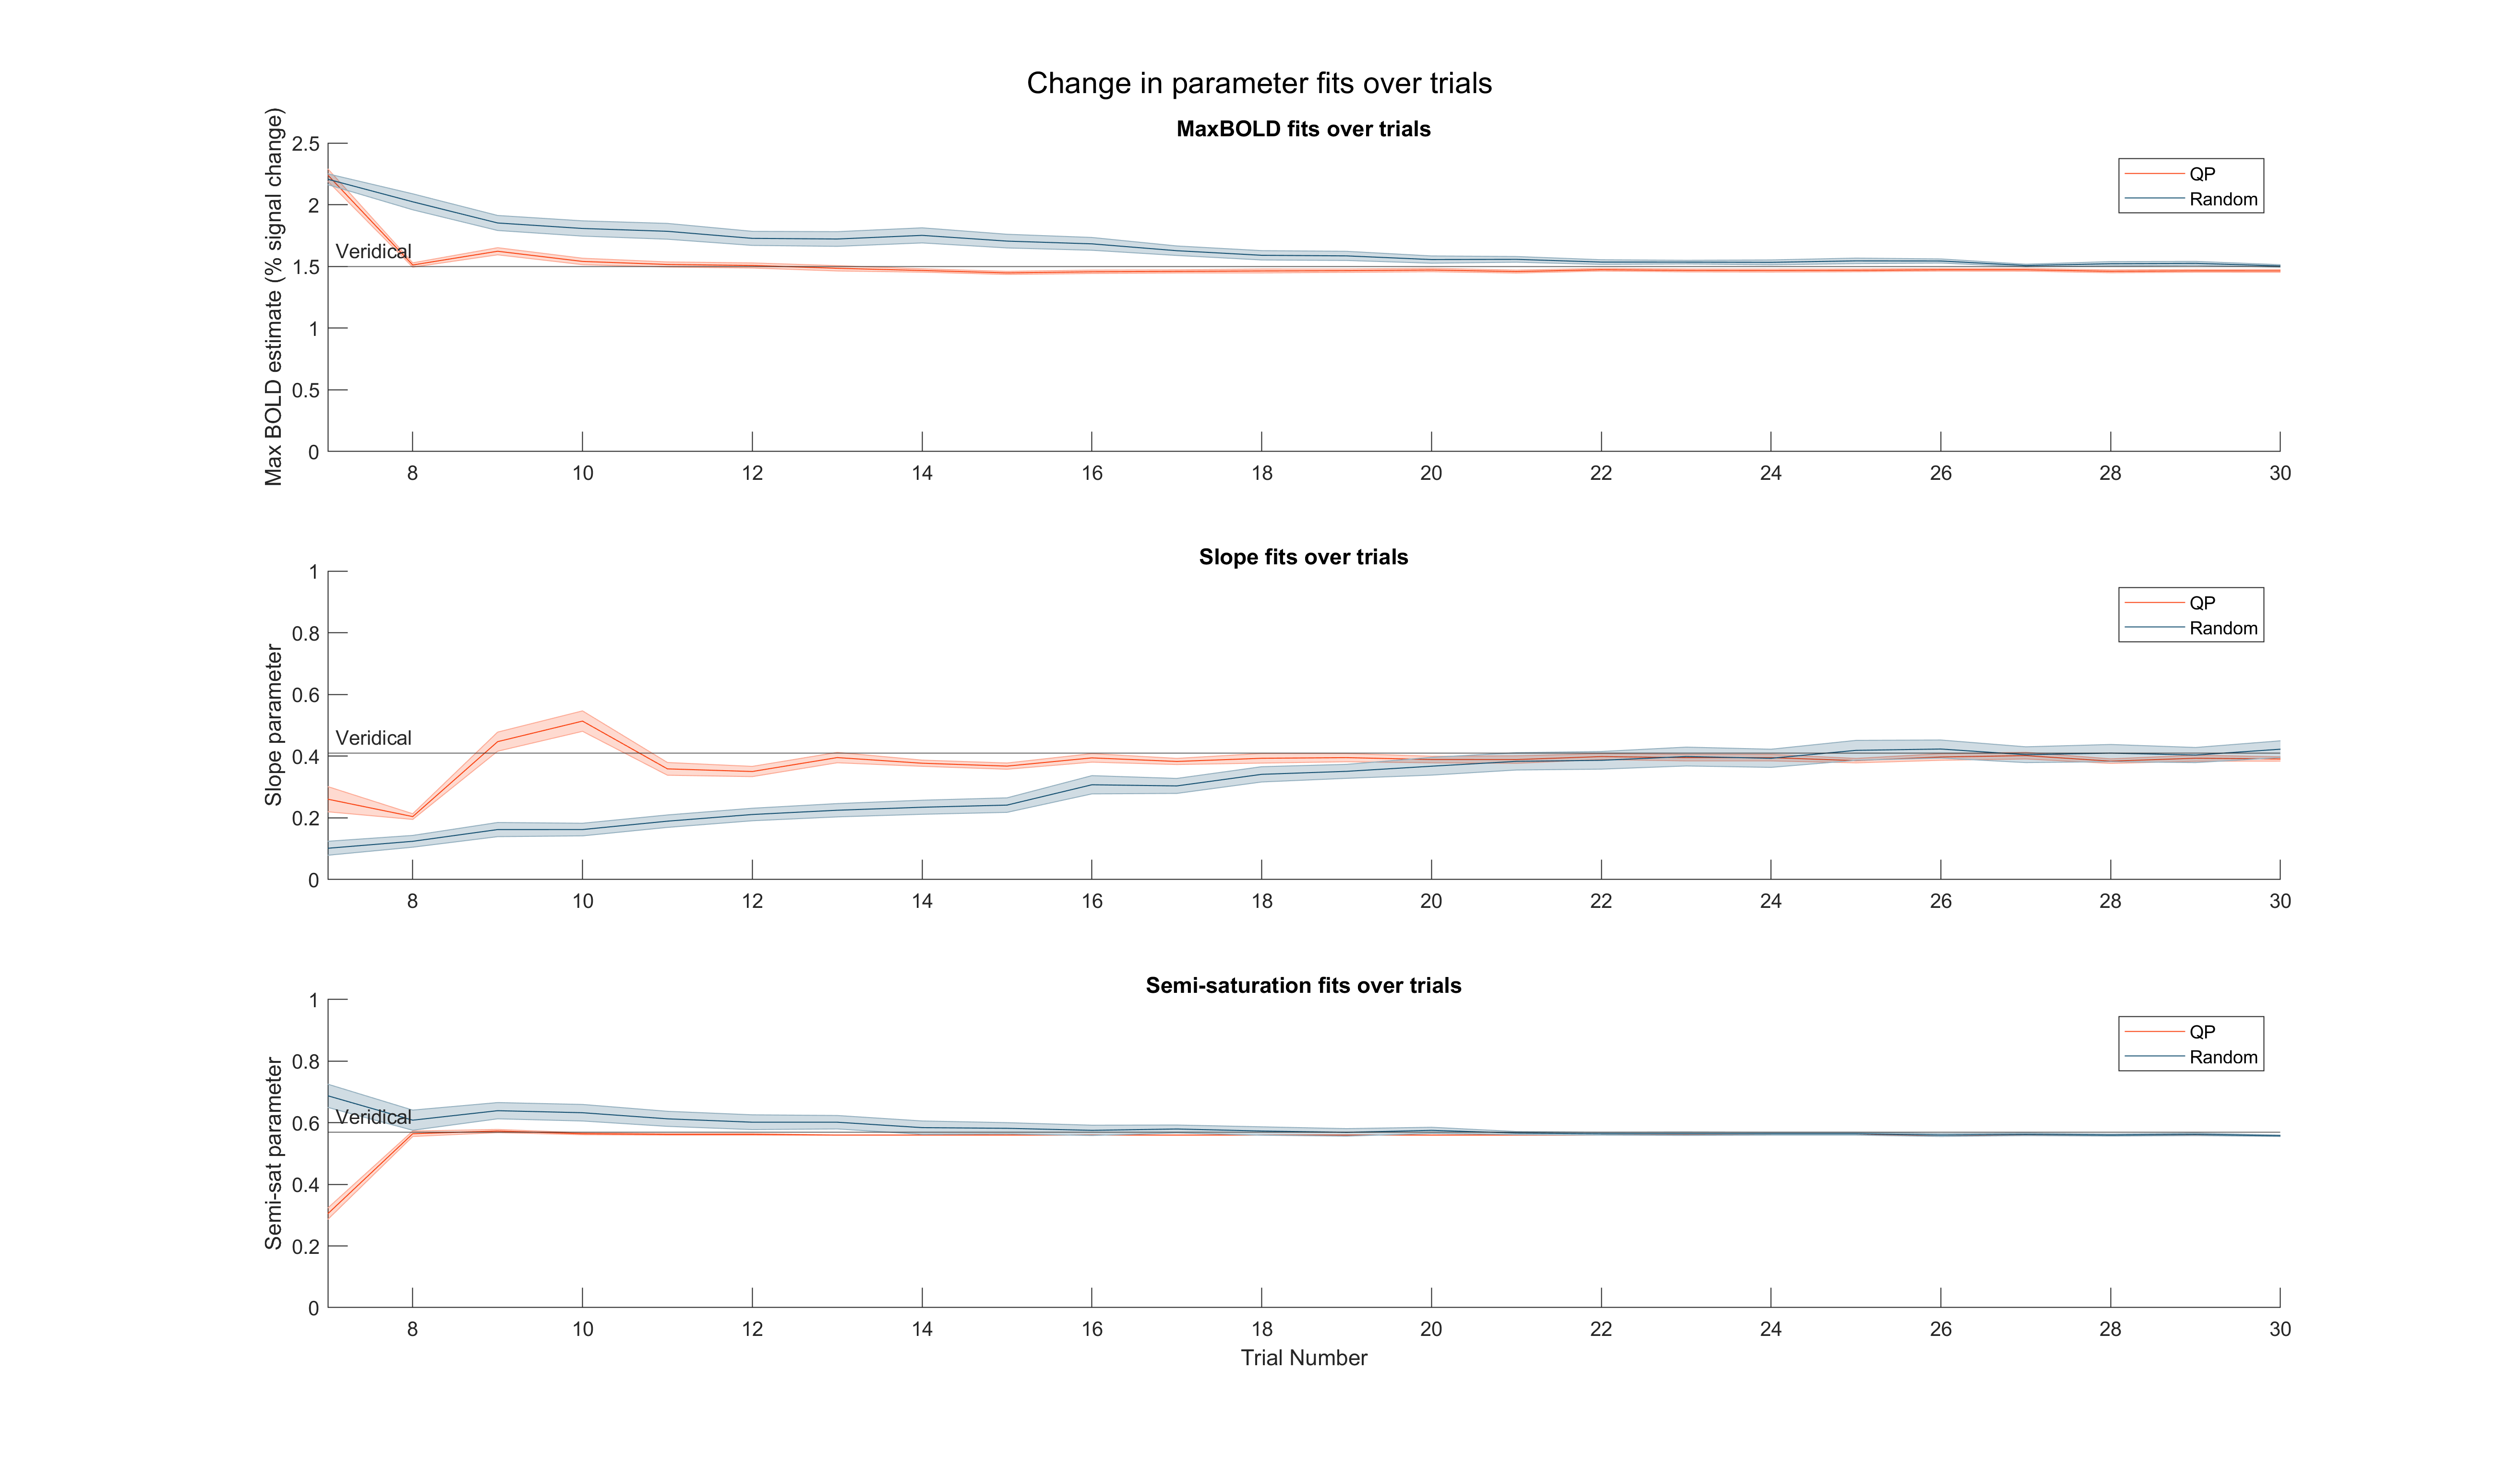
\includegraphics[width=500px]{../results/figs/fig3_7Outcomes_15Noise_12trialLength_800TR} 
  
  }
  
  \caption{Excluding the first 5 trials (which were chosen to be alternating baseline and maximum BOLD trials), we plot the mean (thick line) and standard error (shaded area) estimates for the maximum BOLD estimate (top panel), slope (middle panel) and semi-saturation (bottom panel) averaged over all simulations after each trial. All three parameters are estimated more quickly and with less error when Q+ stimulus selection is used (orange) compared to random stimulus selection (blue).
\newpage}\label{fig:results-figure-firstsims-3}
  \end{figure}




\hypertarget{varying-control-parameters}{%
\subsection{Varying control parameters}\label{varying-control-parameters}}

Q+ improves model fit over random stimulus selection for one set of control parameters, but how does Q+ stimulus selection perform over a range of control parameters? We varied two properties of the experimental design: time to repetition (TR; 800 or 1600 ms) and how long each trial was (8 or 12 seconds). We also varied one property of the reverse model: the number of outcomes categories or bins (7 or 15). Finally, we explored three levels of noise in the response (.15, .45, .75 SDs). These levels could roughly correspond to low, medium, and high noise. (FIGURE XX). The purpose of these set of simulations was to see both how robust the Q+ stimulus selection advantage was and whether any experimental design choices may affect the accuracy of the results.

Table 1 presents the overall findings averaged over each set of 50 simulations.

\begin{lltable}

\begin{TableNotes}[para]
\normalsize{\textit{Note.} Non-parametric t-tests (Wilcoxon signed-rank) comparing each set of simulations for parameter values. TR = Time to repetition.}
\end{TableNotes}

\begin{longtable}{cccccccccc}\noalign{\getlongtablewidth\global\LTcapwidth=\longtablewidth}
\caption{\label{tab:unnamed-chunk-1}Results by simulation parameter sets.}\\
\toprule
 \multicolumn{4}{c}{Parameters} & \multicolumn{6}{c}{Results} \\
\cmidrule(r){1-4} \cmidrule(r){5-10}
Noise & \multicolumn{1}{c}{Bins} & \multicolumn{1}{c}{Trial Length (s)} & \multicolumn{1}{c}{TR} & \multicolumn{1}{c}{qpMean} & \multicolumn{1}{c}{qpSD} & \multicolumn{1}{c}{randMean} & \multicolumn{1}{c}{randSD} & \multicolumn{1}{c}{Z-score} & \multicolumn{1}{c}{p-value}\\
\midrule
\endfirsthead
\caption*{\normalfont{Table \ref{tab:unnamed-chunk-1} continued}}\\
\toprule
 \multicolumn{4}{c}{Parameters} & \multicolumn{6}{c}{Results} \\
\cmidrule(r){1-4} \cmidrule(r){5-10}
Noise & \multicolumn{1}{c}{Bins} & \multicolumn{1}{c}{Trial Length (s)} & \multicolumn{1}{c}{TR} & \multicolumn{1}{c}{qpMean} & \multicolumn{1}{c}{qpSD} & \multicolumn{1}{c}{randMean} & \multicolumn{1}{c}{randSD} & \multicolumn{1}{c}{Z-score} & \multicolumn{1}{c}{p-value}\\
\midrule
\endhead
0.1500 & 7 & 8 & 800 & 0.9952 & 0.0192 & 0.9821 & 0.0498 & 4.8636 & 0.0000\\
0.1500 & 7 & 8 & 1600 & 0.9979 & 0.0021 & 0.9849 & 0.0277 & 3.9191 & 0.0001\\
0.1500 & 7 & 12 & 800 & 0.9986 & 0.0012 & 0.9817 & 0.0348 & 5.1256 & 0.0000\\
0.1500 & 7 & 12 & 1600 & 0.9972 & 0.0030 & 0.9819 & 0.0451 & 1.6097 & 0.1075\\
0.1500 & 15 & 8 & 800 & 0.9976 & 0.0023 & 0.9836 & 0.0363 & 4.4224 & 0.0000\\
0.1500 & 15 & 8 & 1600 & 0.9978 & 0.0023 & 0.9825 & 0.0297 & 6.0631 & 0.0000\\
0.1500 & 15 & 12 & 800 & 0.9971 & 0.0044 & 0.9801 & 0.0628 & 3.4159 & 0.0006\\
0.1500 & 15 & 12 & 1600 & 0.9981 & 0.0020 & 0.9853 & 0.0273 & 5.1462 & 0.0000\\
0.4500 & 7 & 8 & 800 & 0.9829 & 0.0258 & 0.9609 & 0.0787 & 2.4508 & 0.0143\\
0.4500 & 7 & 8 & 1600 & 0.9728 & 0.0391 & 0.9471 & 0.0681 & 1.4718 & 0.1411\\
0.4500 & 7 & 12 & 800 & 0.9767 & 0.0396 & 0.9587 & 0.0504 & 2.9471 & 0.0032\\
0.4500 & 7 & 12 & 1600 & 0.9832 & 0.0297 & 0.9460 & 0.0623 & 4.1260 & 0.0000\\
0.4500 & 15 & 8 & 800 & 0.9880 & 0.0163 & 0.9409 & 0.0700 & 4.9394 & 0.0000\\
0.4500 & 15 & 8 & 1600 & 0.9770 & 0.0462 & 0.9290 & 0.0811 & 4.2018 & 0.0000\\
0.4500 & 15 & 12 & 800 & 0.9886 & 0.0145 & 0.9445 & 0.0759 & 5.3668 & 0.0000\\
0.4500 & 15 & 12 & 1600 & 0.9874 & 0.0096 & 0.9517 & 0.0578 & 3.1746 & 0.0015\\
0.7500 & 7 & 8 & 800 & 0.9084 & 0.0794 & 0.8591 & 0.1446 & 1.5821 & 0.1136\\
0.7500 & 7 & 8 & 1600 & 0.8479 & 0.2067 & 0.8214 & 0.1661 & 1.4925 & 0.1356\\
0.7500 & 7 & 12 & 800 & 0.9143 & 0.1026 & 0.8851 & 0.0894 & 2.0578 & 0.0396\\
0.7500 & 7 & 12 & 1600 & 0.8910 & 0.1960 & 0.8355 & 0.1850 & 3.0850 & 0.0020\\
0.7500 & 15 & 8 & 800 & 0.8474 & 0.2254 & 0.8454 & 0.1540 & 1.5992 & 0.1098\\
0.7500 & 15 & 8 & 1600 & 0.8421 & 0.1743 & 0.7961 & 0.1830 & 1.8303 & 0.0672\\
0.7500 & 15 & 12 & 800 & 0.9044 & 0.1453 & 0.8698 & 0.1392 & 1.9199 & 0.0549\\
0.7500 & 15 & 12 & 1600 & 0.9044 & 0.1596 & 0.8393 & 0.1784 & 2.7541 & 0.0059\\
\bottomrule
\addlinespace
\insertTableNotes
\end{longtable}

\end{lltable}

Table 2 presents the results of ANOVA comparing the three levels.

\begin{table}[tbp]

\begin{center}
\begin{threeparttable}

\caption{\label{tab:unnamed-chunk-2}Results by simulation parameter sets.}

\begin{tabular}{lcccccl}
\toprule
Predictor & \multicolumn{1}{c}{Sum of Squares} & \multicolumn{1}{c}{df} & \multicolumn{1}{c}{Mean.Sq.} & \multicolumn{1}{c}{F} & \multicolumn{1}{c}{p} & \multicolumn{1}{c}{Partial eta squared}\\
\midrule
TR & 0.0586 & 1 & 0.0586 & 0.7693 & 0.3805 & 0.0003\\
fMRI Noise & 5.9027 & 2 & 2.9514 & 38.7407 & 0.0000 & 0.0303\\
Trial Length & 0.1732 & 1 & 0.1732 & 2.2741 & 0.1317 & 0.0009\\
TR*fMRI Noise & 0.1723 & 2 & 0.0862 & 1.1308 & 0.3229 & 0.0009\\
TR*Trial Length & 0.5499 & 1 & 0.5499 & 7.2181 & 0.0073 & 0.0029\\
fMRI Noise*Trial Length & 0.0856 & 2 & 0.0428 & 0.5616 & 0.5704 & 0.0005\\
Error & 182.0005 & 2389 & 0.0762 & NA & NA & 0.4906\\
Total & 188.9453 & 2398 & NA & NA & NA & 0.5000\\
\bottomrule
\addlinespace
\end{tabular}

\begin{tablenotes}[para]
\normalsize{\textit{Note.} ANOVA}
\end{tablenotes}

\end{threeparttable}
\end{center}

\end{table}

\hypertarget{show-an-example-simulated-experiment-with-the-convergence-of-the-adaptive-procedure-upon-the-parameters-of-the-response-function}{%
\subsection{Show an example simulated experiment with the convergence of the adaptive procedure upon the parameter(s) of the response function}\label{show-an-example-simulated-experiment-with-the-convergence-of-the-adaptive-procedure-upon-the-parameters-of-the-response-function}}

\hypertarget{explore-choices-for-the-trial-duration-and-tr-to-find-optimal-experimental-design-for-rapid-and-accurate-parameter-characterization.-examples-how-finely-to-sample-the-stimulus-space-scan-length-number-of-trials-stimulus-duration-forcing-occasional-baseline-trials-to-account-for-1f-drift-in-the-bold-fmri-signal}{%
\subsection{\texorpdfstring{Explore choices for the trial duration and TR to find optimal experimental design for rapid and accurate parameter characterization. Examples: How finely to sample the stimulus space; scan length, number of trials, stimulus duration; Forcing occasional \enquote{baseline} trials to account for 1/f drift in the BOLD fMRI signal}{Explore choices for the trial duration and TR to find optimal experimental design for rapid and accurate parameter characterization. Examples: How finely to sample the stimulus space; scan length, number of trials, stimulus duration; Forcing occasional ``baseline'' trials to account for 1/f drift in the BOLD fMRI signal}}\label{explore-choices-for-the-trial-duration-and-tr-to-find-optimal-experimental-design-for-rapid-and-accurate-parameter-characterization.-examples-how-finely-to-sample-the-stimulus-space-scan-length-number-of-trials-stimulus-duration-forcing-occasional-baseline-trials-to-account-for-1f-drift-in-the-bold-fmri-signal}}

\hypertarget{comparison-of-method-of-constant-stimuli-to-bayesian-adaptive-fmri-for-time-to-achieve-a-given-degree-of-confidence-in-an-experimental-parameter.}{%
\subsection{Comparison of method of constant stimuli to Bayesian adaptive fMRI for time to achieve a given degree of confidence in an experimental parameter.}\label{comparison-of-method-of-constant-stimuli-to-bayesian-adaptive-fmri-for-time-to-achieve-a-given-degree-of-confidence-in-an-experimental-parameter.}}

\hypertarget{discussion}{%
\section{Discussion}\label{discussion}}

\hypertarget{limitations}{%
\subsection{Limitations}\label{limitations}}

\hypertarget{this-is-really-only-useful-if-you-already-have-a-strong-prior-on-the-possible-shape-of-the-response-function.}{%
\subsubsection{This is really only useful if you already have a strong prior on the possible shape of the response function.}\label{this-is-really-only-useful-if-you-already-have-a-strong-prior-on-the-possible-shape-of-the-response-function.}}

\hypertarget{a-great-use-case-is-when-the-distribution-andor-bounds-on-the-parameter-values-for-a-population-is-known-but-the-investigator-now-wishes-to-estimate-the-parameter-value-for-a-particular-individual-under-study.}{%
\subsubsection{A great use case is when the distribution and/or bounds on the parameter values for a population is known, but the investigator now wishes to estimate the parameter value for a particular individual under study.}\label{a-great-use-case-is-when-the-distribution-andor-bounds-on-the-parameter-values-for-a-population-is-known-but-the-investigator-now-wishes-to-estimate-the-parameter-value-for-a-particular-individual-under-study.}}

\hypertarget{extensions}{%
\subsection{Extensions}\label{extensions}}

\hypertarget{model-parameters-that-account-for-variation-across-cortical-space.-could-have-a-model-that-takes-as-input-multiple-time-series-and-then-has-a-parameter-that-describes-systematic-variation-in-responses-across-space-e.g.-retinotopic-mapping.}{%
\subsubsection{Model parameters that account for variation across cortical space. Could have a model that takes as input multiple time-series and then has a parameter that describes systematic variation in responses across space (e.g., retinotopic mapping).}\label{model-parameters-that-account-for-variation-across-cortical-space.-could-have-a-model-that-takes-as-input-multiple-time-series-and-then-has-a-parameter-that-describes-systematic-variation-in-responses-across-space-e.g.-retinotopic-mapping.}}

\hypertarget{could-model-not-just-parameters-for-the-neural-response-but-physiologic-parameters-as-well.-e.g.-the-parameters-that-define-the-shape-of-the-hemodynamic-response-or-saturating-non-linearities-in-the-conversion-of-neural-activity-to-bold-signal.}{%
\subsubsection{Could model not just parameters for the neural response, but physiologic parameters as well. E.g., the parameters that define the shape of the hemodynamic response, or saturating non-linearities in the conversion of neural activity to BOLD signal.}\label{could-model-not-just-parameters-for-the-neural-response-but-physiologic-parameters-as-well.-e.g.-the-parameters-that-define-the-shape-of-the-hemodynamic-response-or-saturating-non-linearities-in-the-conversion-of-neural-activity-to-bold-signal.}}

\hypertarget{results-1}{%
\section{Results}\label{results-1}}

\hypertarget{discussion-1}{%
\section{Discussion}\label{discussion-1}}

\newpage

\hypertarget{references}{%
\section{References}\label{references}}

\begingroup
\setlength{\parindent}{-0.5in}
\setlength{\leftskip}{0.5in}

\hypertarget{refs}{}
\leavevmode\hypertarget{ref-davidh.brainardMQUESTPlusMatlabImplementation2017}{}%
David H. Brainard. (2017). mQUESTPlus: A Matlab implementation of QUEST+.

\leavevmode\hypertarget{ref-watsonQUESTGeneralMultidimensional2017}{}%
Watson, A. B. (2017). QUEST+: A general multidimensional Bayesian adaptive psychometric method. \emph{Journal of Vision}, \emph{17}(3), 10--10. \url{https://doi.org/10.1167/17.3.10}

\leavevmode\hypertarget{ref-watsonQuestBayesianAdaptive1983}{}%
Watson, A. B., \& Pelli, D. G. (1983). Quest: A Bayesian adaptive psychometric method. \emph{Perception \& Psychophysics}, \emph{33}(2), 113--120. \url{https://doi.org/10.3758/BF03202828}

\endgroup


\end{document}
